\documentclass[]{article}

% Imported Packages
%------------------------------------------------------------------------------
\usepackage{amssymb}
\usepackage{amstext}
\usepackage{amsthm}
\usepackage{amsmath}
\usepackage{enumerate}
\usepackage{fancyhdr}
\usepackage[margin=1in]{geometry}
\usepackage{graphicx}
%\usepackage{extarrows}
%\usepackage{setspace}
%\usepackage{xcolor}
\usepackage{color}
%------------------------------------------------------------------------------

% Header and Footer
%------------------------------------------------------------------------------
\pagestyle{plain}  
\renewcommand\headrulewidth{0.4pt}                                      
\renewcommand\footrulewidth{0.4pt}                                    
%------------------------------------------------------------------------------

% Title Details
%------------------------------------------------------------------------------
\title{Deliverable \#1 Template : Software Requirement Specification (SRS)}
\author{SE 3A04: Software Design II -- Large System Design}
\date{18 February 2024}
                            
%------------------------------------------------------------------------------

% Document
%------------------------------------------------------------------------------
\begin{document}

\maketitle	
\noindent{\bf Tutorial Number:} T01\\
{\bf Group Number:} G07 \\
{\bf Group Members:} 
\begin{itemize}
	\item Awurama Nyarko
	\item Chelsea Maramot
 	\item Harrison Chiu
  	\item Khushi Bhojane
   	\item Sumanya Gulati
\end{itemize}

\section*{IMPORTANT NOTES}
\begin{itemize}
	\item Be sure to include all sections of the template in your document regardless whether you have something to write for each or not
	\begin{itemize}
		\item If you do not have anything to write in a section, indicate this by the \emph{N/A}, \emph{void}, \emph{none}, etc.
	\end{itemize}
	\item Uniquely number each of your requirements for easy identification and cross-referencing
	\item Highlight terms that are defined in Section~1.3 (\textbf{Definitions, Acronyms, and Abbreviations}) with \textbf{bold}, \emph{italic} or \underline{underline}
	\item For Deliverable 1, please highlight, in some fashion, all (you may have more than one) creative and innovative features. Your creative and innovative features will generally be described in Section~2.2 (\textbf{Product Functions}), but it will depend on the type of creative or innovative features you are including.
\end{itemize}

\newpage
\section{Introduction}
\label{sec:introduction}
% Begin Section

\begin{itemize}
	\item Provide an overview of the document/SRS.
\end{itemize}


\subsection{Purpose}
\label{sub:purpose}
% Begin SubSection
\begin{itemize}
	\item Specify the purpose of the SRS.
	\item Specify the intended audience for the SRS.
\end{itemize}
% End SubSection

\subsection{Scope}
\label{sub:scope}
% Begin SubSection
\begin{itemize}
	\item Identify the software product(s) to be produced, and name each (e.g., Host DBMS, Report Generator, etc.)
	\item Explain what the software product(s) will do (and, if necessary, also state what they will not do).
	\item Describe the application of the software being specified, including relevant benefits, objectives, and goals.
%	\item Be consistent with similar statements in higher-level specifications (e.g., the system requirements specification), if they exist
\end{itemize}
% End SubSection

\subsection{Definitions, Acronyms, and Abbreviations}
\label{sub:definitions_acronyms_and_abbreviations}
% Begin SubSection
\begin{itemize}
	\item Provide the definitions of all terms, acronyms, and abbreviations required to properly interpret the SRS.
	\item This should be in alphabetical order.
\end{itemize}
% End SubSection

\subsection{References}
\label{sub:references}
% Begin SubSection
\begin{itemize}
	\item Provide a complete list of all documents referenced elsewhere in the SRS.
	\item Identify each document by title, report number (if applicable), date, and publishing organization.
	\item Specify the sources from which the references can be obtained.
	\item Order this list in some sensible manner (alphabetical by author, or something else that makes more sense).
\end{itemize}
% End SubSection

\subsection{Overview}
\label{sub:overview}
% Begin SubSection
\begin{itemize}
	\item Describe what the remainder of the document/SRS contains.\\
	(e.g. "Section 2 discusses...Section 3...")
%	\item Explain how the SRS is organized
\end{itemize}
% End SubSection

% End Section

\section{Overall Product Description}
\label{sec:overall_description}
% Begin Section

\subsection{Product Perspective}
\label{sub:product_perspective}
% Begin SubSection
SecureChat is a chat-based application developed for a specific organization and its employees. Similar, commerically available tools incude popular workplace collaboration softwares like Slack, Microsoft Teams and Discord as well as popular instant messaging services such as WhatsApp, Facebook Messenger and Telegram. SecureChat is designed to be an amalgamation of both of these services and provide secure communication channels for its users.\\
The app allows users to communicate using individual user-to-user chats or group chats involving multiple users (with a maximum limit of 50). To allow for seamless communication, SecureChat has file sharing functionality that allows users to modify file permissions and share them securely in individual or group chats. Although, user profiles can only be created or deleted by administration for security measures, users are able to modify their personal details as well as details and permissions for group chats (such as name, description and more). Most of these features can be found in the workplace collaboration softwares and instant messaging services listed above.\\
The product is a standalone application that is expected to be a part of the organization's existing IT infrastructure. In term of security measures, the app interacts with a KDC server that generates and sends all keys to users at the starting of all secure communication sessions. For regulatory and compliance concerns, the chat history logs for all communication sessions including details such as user profiles, time stamps and message content are securely stored on a server for 2 years from the original timestamp.\\
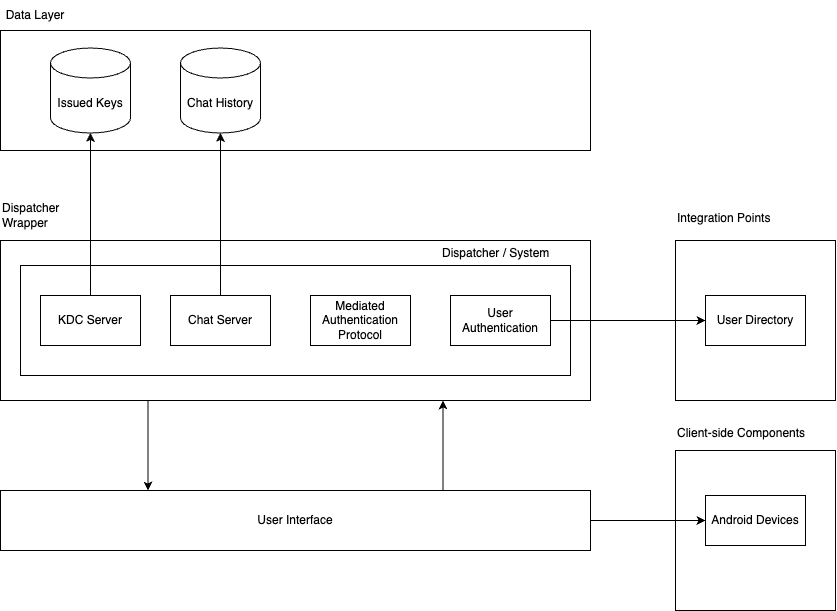
\includegraphics{system-diagram.png}
\caption{Figure 1. System Diagram}
% End SubSection

\subsection{Product Functions}
\label{sub:product_functions}
% Begin SubSection
\begin{itemize}
	\item Provide a \emph{summary} of the major functions that the software will perform.
	\begin{itemize}
		\item \textbf{Example}: An SRS for an accounting program may use this part to address customer account maintenance, customer statement, and invoice preparation without mentioning the vast amount of detail that each of those functions requires.
	\end{itemize}
	\item Functions should be organized in a way that makes the list of functions understandable to the customer or to anyone else reading the document for the first time 
	\item Present the functions in a list format - each item should be one function, with a brief description of it
	\item Textual or graphical methods can be used to show the different functions and their relationships
	\begin{itemize}
		\item Such a diagram is not intended to show a design of a product, but simply shows the logical relationships among variables
	\end{itemize} 
\end{itemize}
% End SubSection

\subsection{User Characteristics}
\label{sub:user_characteristics}
% Begin SubSection
SecureChat is intended to be a user-friendly app designed for the current employees of a specific organization. As a result, the following are the minimum qualifications expected from all users:
\begin{itemize}
	\item Education Level: Basic literacy skills
 	\begin{itemize}
  		\item Users are expected to possess basic English literacy skills, specifically reading and writing.
    		\item The interface of the app is intended to be intuitive and user-friendly with clear instructions provided for using security features. This means that users with varying levels of education should be able to use the app.
      	\end{itemize}
 	\item Technical Expertise: Basic smartphone navigation skills
  	\begin{itemize}
   		\item Users are expected to have basic smartphone (specifically, Android) navigation skills.
     		\item Although not mandatory, ideally, users should have basic security awareness about concepts such as password security, phishing awareness, data encryption and more.
       	\end{itemize}
  	\item Experience: Familiarity with chat-based services
   	\begin{itemize}
    		\item Users are expected to possess prior experience using commonly used communication tools and technologies. This can include familiarity with instant messaging apps, email services or collaboration platforms such as Microsoft Teams, Slack, Discord etc.
      	\end{itemize}
   	\item Security Clearance: Currently employed by the organization
    	\begin{itemize}
     		\item Users must be currently employed by the organization and be permitted to use the application.
       		\item Users are expected to possess an Android device issued by the organization.
	\end{itemize}
\end{itemize}
% End SubSection

\subsection{Constraints}
\label{sub:constraints}
% Begin SubSection
\begin{itemize}
	\item \emph{Budget}: The allocated budget of the project will directly impact the technologies developers can use as well as the features that can be included in the initial launch of the application. As of the latest update to this SRS document, the budget allocated to the project is 0 CAD.
 	\item \emph{Project Timeline}: Time allocated to the development of the application will affect the scale of the project and the scope of features deployed.
  	\item \emph{Regulatory Compliance}: The application must adhere to relevant regulatory requirements including but not limited to, PIPEDA and industry-specific data storage guidelines for periodic audits.
   	\item \emph{Compatibility Requirements}: The application must be compatible with the organization's existing IT infrastructure and network configurations. Additionally, it must compatible with Android devices.
\end{itemize}
% End SubSection

\subsection{Assumptions and Dependencies}
\label{sub:assumptions_and_dependencies}
% Begin SubSection
\begin{itemize}
	\item It is assumed that the app can only be used by current employees and that a user's access to the app must be revoked when and if they leave the organization.
 	\item It is assumed that all users of the app have access to Android devices issued by the organization.
  	\item It is assumed that users will have reliable internet connectivity at all times while using the application. Currently, offline capabilities for users with limited or intermittent internet access is not implemented.	
   	\item It is assumed that the app is used only by employees who reside in Canada. Usage of the app outside of the country is assumed to be restricted.
    	\item It is assumed that all user profiles must be created/deleted and approved by the administration. Users cannot create new profiles or delete existing profiles on their own.
    	\item Innovative feature: Users are allowed to send disappearing messages for as an enhanced security measure. 
\end{itemize}
Other dependencies that directly impact the app and in case of failure could require a change to the requirements include:
\begin{itemize}
	\item The app must be compatible with the latest available version of Android.
 	\item Since the functionality of the app relies on the availability and proper functioning of a KDC server, any downtime or unexpected disruptions to the server could impact the user's ability to authenticate and securely communicate using the application.
\end{itemize}
% End SubSection

\subsection{Apportioning of Requirements}
\label{sub:apportioning_of_requirements}
% Begin SubSection
\begin{itemize}
	\item Integration with third-party services
 	\begin{itemize}
  		\item The app can have possible integrations with third-party services like email services, video conferencing platforms and more.
    	\end{itemize}
     	\item Offline mode
      	\begin{itemize}
  		\item Currently, the app relies on internet connectivity for receiving keys from the KDC server and authenticating users for each communication session. Alternate methods for authentication that reduce dependency on internet connectivity can be explored in the future.
    	\end{itemize}
     	\item Advanced search and filtering
      	\begin{itemize}
       		\item Functionality for filtering through conversations using keywords and searching for specific files shared within a chat can be added in future versions of the application.
	\end{itemize}
  	\item Additional security measures
   	\begin{itemize}
    		\item Measures such as two-factor authentication, data loss preventation and more can be deferred to subsequent releases.
      	\end{itemize}
\end{itemize}
% End SubSection

% End Section
\section{Use Case Diagram}
\label{sec:use_case_diagram}
% Begin Section
\begin{itemize}
	\item Provide the use case diagram for the system being developed.
	\item You do not need to provide the textual description of any of the use cases here (these will be specified under "Highlights of Functional Requirements").
%	\item Provide \emph{one} use case diagram for the most important Business Event.
%	\item The text of all use cases will be specified under "Highlights of Functional Requirements"
\end{itemize}
%In this section, select the most important Business Event that your system responds to and give its use case diagram.  Only one use case diagram is needed.  Give a brief textual description of the use case without repeating what is in the scenarios of the corresponding Business Event.

%
%
%
%This section should provide a use case diagram for your application. 
%\begin{enumerate}[a)]
%	\item Each use case appearing in the diagram should be accompanied by a text description. 
%\end{enumerate}
%% End Section

\section{Highlights of Functional Requirements}
\label{sec:functional_requirements}
% Begin Section
\begin{itemize}
	\item Specify all use cases (or other scenarios triggered by other events), organized by Business Event. 
	\item For each Business Event, show the scenario from every Viewpoint. You should have the same set of Viewpoints across all Business Events. If a Viewpoint doesn't participate, write N/A so we know you considered it still. You can choose how to present this - keep in mind it should be easy to follow. 
	\item At the end, combine them all into a Global Scenario.
	%\item Specify the "use cases" (or other triggering events) organized by Business Event. (The Global Scenario is what you might think of as a use case). Be sure to consider Business Events that aren't just triggered by users with goals (e.g. something happens in the environment that your system needs to respond to)
	\item Your focus should be on what the system needs to do, not how to do it. Specify it in enough detail that it clearly specifies what needs to be accomplished, but not so detailed that you start programming or making design decisions.
	\item Keep the length of each use case (Global Scenario) manageable. If it's getting too long, split into sub-cases.
	\item You are \emph{not} specifying a complete and consistent set of functional requirements here. (i.e. you are providing them in the form of use cases/global scenarios, not a refined list). For the purpose of this project, you do not need to reduce them to a list; the global scenarios format is all you need.
	\item Red text below is just to highlight where you need to insert a scenario - don't actually write it all in red.
\end{itemize}

\noindent {\bf Main Business Events:} List out all the main business events you are presenting. If you sub-divided into smaller ones, you don't need to include the smaller ones in this list.\\

\noindent {\bf Viewpoints:} List out all the viewpoints you will be considering.\\

\noindent {\bf Interpretation:} Specify any liberties you took in interpreting business events, if necessary.\\

\begin{enumerate}[{\bf BE1.}]
	\item Business Event Name \#1
		\begin{enumerate}[{\bf VP1.}]
			\item Viewpoint Name \#1 \\
				\textcolor{red}{Insert Scenario Here}
			\item Viewpoint Name \#2 \\
				\textcolor{red}{Insert Scenario Here}
		\end{enumerate}
		{\bf Global Scenario:}\\
		\textcolor{red}{Insert Scenario Here}
	\item Business Event Name \#2
	\begin{enumerate}[{\bf VP1.}]
		\item Viewpoint Name \#1 \\
		\textcolor{red}{Insert Scenario Here}
		\item Viewpoint Name \#2 \\
		\textcolor{red}{Insert Scenario Here}
	\end{enumerate}
	{\bf Global Scenario:}\\
	\textcolor{red}{Insert Scenario Here}
\end{enumerate}

%	Below, we organize by Business Event.
%	\begin{enumerate}[{BE}1.]
%		\item Business Event name
%		\begin{enumerate}[{VP1}.1]
%			\item Viewpoint name \newline
%			\noindent\fbox{%
%				\parbox{0.5\textwidth}{%
%					\begin{itemize}
%						\item {\bf $S_{1}$:} Initial response of the system to the Business Event
%						\item {\bf $E_{1}$:}  Reaction of the environment to $S_{1}$
%						\item {\bf $S_{2}$:}  Response of the system to $E_{1}$
%						\item {\bf $E_{2}$:}  Reaction of the environment to $S_{2}$
%						\item[] $\cdots$
%						\item {\bf $S_{n}$:}  Response of the system to $E_{(n-1)}$
%						\item {\bf $E_{n}$:}  Reaction of the environment to $E_{(n-1)}$
%						\item {\bf $S_{(n+1)}$:} Final response of the system concluding its function regarding the Business Event
%					\end{itemize}
%				}%
%			}
%			\item Viewpoint name\newline
%			\noindent\fbox{%
%				\parbox{0.5\textwidth}{%
%					\begin{itemize}
%						\item {\bf $S_{1}$:} Initial response of the system to the Business Event
%						\item {\bf $E_{1}$:}  Reaction of the environment to $S_{1}$
%						\item {\bf $S_{2}$:}  Response of the system to $E_{1}$
%						\item {\bf $E_{2}$:}  Reaction of the environment to $S_{2}$
%						\item[] $\cdots$
%						\item {\bf $S_{k}$:}  Response of the system to $E_{(k-1)}$
%						\item {\bf $E_{k}$:}  Reaction of the environment to $E_{(k-1)}$
%						\item {\bf $S_{(k+1)}$:} Final response of the system concluding its function regarding the Business Event
%					\end{itemize}
%				}%
%			}
%			\item \dots
%			\item \dots
%			\item \dots
%			\item[\dots]
%		\end{enumerate}	
%		\item[] {\bf Global Scenario of {\it Business Event Name}:} It is the scenario corresponding to the integration of all the above scenarios from the different Viewpoints of the Business Event BE1.\newline
%		\noindent\fbox{%
%			\parbox{0.5\textwidth}{%
%				\begin{itemize}
%					\item {\bf $S_{1}$:} Initial response of the system to the Business Event
%					\item {\bf $E_{1}$:}  Reaction of the environment to $S_{1}$
%					\item {\bf $S_{2}$:}  Response of the system to $E_{1}$
%					\item {\bf $E_{2}$:}  Reaction of the environment to $S_{2}$
%					\item[] $\cdots$
%					\item {\bf $S_{m}$:}  Response of the system to $E_{(m-1)}$
%					\item {\bf $E_{m}$:}  Reaction of the environment to $E_{(m-1)}$
%					\item {\bf $S_{(m+1)}$:} Final response of the system concluding its function regarding the Business Event
%				\end{itemize}
%			}%
%		}	
%		%\end{enumerate}
%		\item Business Event name
%		\begin{enumerate}[{VP1}.1]
%			\item Viewpoint name \newline
%			\noindent\fbox{%
%				\parbox{0.5\textwidth}{%
%					\begin{itemize}
%						\item {\bf $S_{1}$:} Initial response of the system to the Business Event
%						\item {\bf $E_{1}$:}  Reaction of the environment to $S_{1}$
%						\item {\bf $S_{2}$:}  Response of the system to $E_{1}$
%						\item {\bf $E_{2}$:}  Reaction of the environment to $S_{2}$
%						\item[] $\cdots$
%						\item {\bf $S_{n'}$:}  Response of the system to $E_{(n'-1)}$
%						\item {\bf $E_{n'}$:}  Reaction of the environment to $E_{(n'-1)}$
%						\item {\bf $S_{(n'+1)}$:} Final response of the system concluding its function regarding the Business Event
%					\end{itemize}
%				}%
%			}
%			\item Viewpoint name\newline
%			\noindent\fbox{%
%				\parbox{0.5\textwidth}{%
%					\begin{itemize}
%						\item {\bf $S_{1}$:} Initial response of the system to the Business Event
%						\item {\bf $E_{1}$:}  Reaction of the environment to $S_{1}$
%						\item {\bf $S_{2}$:}  Response of the system to $E_{1}$
%						\item {\bf $E_{2}$:}  Reaction of the environment to $S_{2}$
%						\item[] $\cdots$
%						\item {\bf $S_{k'}$:}  Response of the system to $E_{(k'-1)}$
%						\item {\bf $E_{k'}$:}  Reaction of the environment to $E_{(k'-1)}$
%						\item {\bf $S_{(k'+1)}$:} Final response of the system concluding its function regarding the Business Event
%					\end{itemize}
%				}%
%			}
%			\item \dots
%			\item \dots
%			\item \dots
%			\item[\dots]
%		\end{enumerate}	
%		\item[] {\bf Global Scenario of {\it Business Event Name}:} It is the scenario corresponding to the integration of all the above scenarios from the different Viewpoints of the Business Event BE2.\newline
%		\noindent\fbox{%
%			\parbox{0.5\textwidth}{%
%				\begin{itemize}
%					\item {\bf $S_{1}$:} Initial response of the system to the Business Event
%					\item {\bf $E_{1}$:}  Reaction of the environment to $S_{1}$
%					\item {\bf $S_{2}$:}  Response of the system to $E_{1}$
%					\item {\bf $E_{2}$:}  Reaction of the environment to $S_{2}$
%					\item[] $\cdots$
%					\item {\bf $S_{m'}$:}  Response of the system to $E_{(m'-1)}$
%					\item {\bf $E_{m'}$:}  Reaction of the environment to $E_{(m'-1)}$
%					\item {\bf $S_{(m'+1)}$:} Final response of the system concluding its function regarding the Business Event
%				\end{itemize}
%			}%
%		}		
%	\end{enumerate}

%End Section

\section{Non-Functional Requirements}
\label{sec:non-functional_requirements}


\begin{itemize}
	\item For each non-functional requirement, provide a justification/rationale for it.\\
	{\bf Example:} \\
	SC1. \emph{The device should not explode in a customer’s pocket.}\\
	{\bf Rationale:} Other companies have had issues with the batteries they used in their phones randomly exploding [insert citation]. This causes a safety issue, as the phone is often carried in a person's hand or pocket.	
	\item If you need to make a guess because you couldn't really talk to stakeholders, you can say "We imagined stakeholders would want...because..."
	\item Each requirement should have a unique label/number for it.
	\item In the list below, if a particular section doesn't apply, just write N/A so we know you considered it.
\end{itemize}

% Begin Section
\subsection{Look and Feel Requirements}
\label{sub:look_and_feel_requirements}
% Begin SubSection

\subsubsection{Appearance Requirements}
\label{ssub:appearance_requirements}
% Begin SubSubSection
\begin{enumerate}[{LF-A}1. ]
	\item 
\end{enumerate}
% End SubSubSection

\subsubsection{Style Requirements}
\label{ssub:style_requirements}
% Begin SubSubSection
\begin{enumerate}[{LF-S}1. ]
	\item 
\end{enumerate}
% End SubSubSection

% End SubSection

\subsection{Usability and Humanity Requirements}
\label{sub:usability_and_humanity_requirements}
% Begin SubSection

\subsubsection{Ease of Use Requirements}
\label{ssub:ease_of_use_requirements}
% Begin SubSubSection
\begin{enumerate}[{UH-EOU}1. ]
	\item 
\end{enumerate}
% End SubSubSection

\subsubsection{Personalization and Internationalization Requirements}
\label{ssub:personalization_and_internationalization_requirements}
% Begin SubSubSection
\begin{enumerate}[{UH-PI}1. ]
	\item 
\end{enumerate}
% End SubSubSection

\subsubsection{Learning Requirements}
\label{ssub:learning_requirements}
% Begin SubSubSection
\begin{enumerate}[{UH-L}1. ]
	\item 
\end{enumerate}
% End SubSubSection

\subsubsection{Understandability and Politeness Requirements}
\label{ssub:understandability_and_politeness_requirements}
% Begin SubSubSection
\begin{enumerate}[{UH-UP}1. ]
	\item 
\end{enumerate}
% End SubSubSection

\subsubsection{Accessibility Requirements}
\label{ssub:accessibility_requirements}
% Begin SubSubSection
\begin{enumerate}[{UH-A}1. ]
	\item 
\end{enumerate}
% End SubSubSection

% End SubSection

\subsection{Performance Requirements}
\label{sub:performance_requirements}
% Begin SubSection

\subsubsection{Speed and Latency Requirements}
\label{ssub:speed_and_latency_requirements}
% Begin SubSubSection
\begin{enumerate}[{PR-SL}1. ]
	\item 
\end{enumerate}
% End SubSubSection

\subsubsection{Safety-Critical Requirements}
\label{ssub:safety_critical_requirements}
% Begin SubSubSection
\begin{enumerate}[{PR-SC}1. ]
	\item 
\end{enumerate}
% End SubSubSection

\subsubsection{Precision or Accuracy Requirements}
\label{ssub:precision_or_accuracy_requirements}
% Begin SubSubSection
\begin{enumerate}[{PR-PA}1. ]
	\item 
\end{enumerate}
% End SubSubSection

\subsubsection{Reliability and Availability Requirements}
\label{ssub:reliability_and_availability_requirements}
% Begin SubSubSection
\begin{enumerate}[{PR-RA}1. ]
	\item 
\end{enumerate}
% End SubSubSection

\subsubsection{Robustness or Fault-Tolerance Requirements}
\label{ssub:robustness_or_fault_tolerance_requirements}
% Begin SubSubSection
\begin{enumerate}[{PR-RFT}1. ]
	\item 
\end{enumerate}
% End SubSubSection

\subsubsection{Capacity Requirements}
\label{ssub:capacity_requirements}
% Begin SubSubSection
\begin{enumerate}[{PR-C}1. ]
	\item 
\end{enumerate}
% End SubSubSection

\subsubsection{Scalability or Extensibility Requirements}
\label{ssub:scalability_or_extensibility_requirements}
% Begin SubSubSection
\begin{enumerate}[{PR-SE}1. ]
	\item 
\end{enumerate}
% End SubSubSection

\subsubsection{Longevity Requirements}
\label{ssub:longevity_requirements}
% Begin SubSubSection
\begin{enumerate}[{PR-L}1. ]
	\item 
\end{enumerate}
% End SubSubSection

% End SubSection

\subsection{Operational and Environmental Requirements}
\label{sub:operational_and_environmental_requirements}
% Begin SubSection

\subsubsection{Expected Physical Environment}
\label{ssub:expected_physical_environment}
% Begin SubSubSection
\begin{enumerate}[{OE-EPE}1. ]
	\item 
\end{enumerate}
% End SubSubSection

\subsubsection{Requirements for Interfacing with Adjacent Systems}
\label{ssub:requirements_for_interfacing_with_adjacent_systems}
% Begin SubSubSection
\begin{enumerate}[{OE-IA}1. ]
	\item 
\end{enumerate}
% End SubSubSection

\subsubsection{Productization Requirements}
\label{ssub:productization_requirements}
% Begin SubSubSection
\begin{enumerate}[{OE-P}1. ]
	\item 
\end{enumerate}
% End SubSubSection

\subsubsection{Release Requirements}
\label{ssub:release_requirements}
% Begin SubSubSection
\begin{enumerate}[{OE-R}1. ]
	\item 
\end{enumerate}
% End SubSubSection

% End SubSection

\subsection{Maintainability and Support Requirements}
\label{sub:maintainability_and_support_requirements}
% Begin SubSection

\subsubsection{Maintenance Requirements}
\label{ssub:maintenance_requirements}
% Begin SubSubSection
\begin{enumerate}[{MS-M}1. ]
	\item 
\end{enumerate}
% End SubSubSection

\subsubsection{Supportability Requirements}
\label{ssub:supportability_requirements}
% Begin SubSubSection
\begin{enumerate}[{MS-S}1. ]
	\item 
\end{enumerate}
% End SubSubSection

\subsubsection{Adaptability Requirements}
\label{ssub:adaptability_requirements}
% Begin SubSubSection
\begin{enumerate}[{MS-A}1. ]
	\item 
\end{enumerate}
% End SubSubSection

% End SubSection

\subsection{Security Requirements}
\label{sub:security_requirements}
% Begin SubSection

\subsubsection{Access Requirements}
\label{ssub:access_requirements}
% Begin SubSubSection
\begin{enumerate}[{SR-AC}1. ]
	\item 
\end{enumerate}
% End SubSubSection

\subsubsection{Integrity Requirements}
\label{ssub:integrity_requirements}
% Begin SubSubSection
\begin{enumerate}[{SR-INT}1. ]
	\item 
\end{enumerate}
% End SubSubSection

\subsubsection{Privacy Requirements}
\label{ssub:privacy_requirements}
% Begin SubSubSection
\begin{enumerate}[{SR-P}1. ]
	\item 
\end{enumerate}
% End SubSubSection

\subsubsection{Audit Requirements}
\label{ssub:audit_requirements}
% Begin SubSubSection
\begin{enumerate}[{SR-AU}1. ]
	\item 
\end{enumerate}
% End SubSubSection

\subsubsection{Immunity Requirements}
\label{ssub:immunity_requirements}
% Begin SubSubSection
\begin{enumerate}[{SR-IM}1. ]
	\item 
\end{enumerate}
% End SubSubSection

% End SubSection

\subsection{Cultural and Political Requirements}
\label{sub:cultural_and_political_requirements}
% Begin SubSection

\subsubsection{Cultural Requirements}
\label{ssub:cultural_requirements}
% Begin SubSubSection
\begin{enumerate}[{CP-C}1. ]
	\item 
\end{enumerate}
% End SubSubSection

\subsubsection{Political Requirements}
\label{ssub:political_requirements}
% Begin SubSubSection
\begin{enumerate}[{CP-P}1. ]
	\item 
\end{enumerate}
% End SubSubSection

% End SubSection

\subsection{Legal Requirements}
\label{sub:legal_requirements}
% Begin SubSection

\subsubsection{Compliance Requirements}
\label{ssub:compliance_requirements}
% Begin SubSubSection
\begin{enumerate}[{LR-COMP}1. ]
	\item 
\end{enumerate}
% End SubSubSection

\subsubsection{Standards Requirements}
\label{ssub:standards_requirements}
% Begin SubSubSection
\begin{enumerate}[{LR-STD}1. ]
	\item 
\end{enumerate}
% End SubSubSection

% End SubSection

% End Section

\appendix
\section{Division of Labour}
\label{sec:division_of_labour}
% Begin Section
Include a Division of Labour sheet which indicates the contributions of each team member. This sheet must be signed by all team members.
% End Section

%\newpage
%\section*{IMPORTANT NOTES}
%\begin{itemize}
%	\item Be sure to include all sections of the template in your document regardless whether you have something to write for each or not
%	\begin{itemize}
%		\item If you do not have anything to write in a section, indicate this by the \emph{N/A}, \emph{void}, \emph{none}, etc.
%	\end{itemize}
%	\item Uniquely number each of your requirements for easy identification and cross-referencing
%	\item Highlight terms that are defined in Section~1.3 (\textbf{Definitions, Acronyms, and Abbreviations}) with \textbf{bold}, \emph{italic} or \underline{underline}
%	\item For Deliverable 1, please highlight, in some fashion, all (you may have more than one) creative and innovative features. Your creative and innovative features will generally be described in Section~2.2 (\textbf{Product Functions}), but it will depend on the type of creative or innovative features you are including.
%\end{itemize}


\end{document}
%------------------------------------------------------------------------------
